\documentclass[withoutpreface,bwprint]{cumcmthesis}
\usepackage{cumcm2026}
\usepackage{url}
\graphicspath{{figures/}}

% 未完成内容的醒目标记，定稿前搜索 "TODO" 全部清理/替换
\newcommand{\TODO}[1]{\textcolor{red}{\textbf{[待补充：#1]}}}

\title{微网与外部电网电力调控策略——基于线性规划的计划购电与储能协同优化模型}
\tihao{C}
\baominghao{\TODO{参赛队编号}}
\schoolname{\TODO{学校名称}}
\membera{\TODO{队员1}}
\memberb{\TODO{队员2}}
\memberc{\TODO{队员3}}
\supervisor{ }
\yearinput{2026}
\monthinput{9}
\dayinput{13}

\begin{document}

\maketitle

\begin{abstract}
微网通过光伏发电与储能设备的协同调度，在满足小区负载的前提下，利用外网电价
的时段差异降低购电费用。本文围绕"微网与外部电网电力调控策略"问题，建立了
以线性规划（LP）为核心的日前购电与储能协同优化模型，并针对全年逐日调度、
紧急购电机制等问题展开分析。

针对\textbf{问题一}，在电价、负荷已知且光伏预测数据视为准确的单日场景下，
以每 10 分钟为决策粒度，建立了以全天购电费最小为目标、以电力平衡与储能
状态（SOC）递推为核心约束的线性规划模型，并要求储能在 0:00 与 24:00 电量
相等。使用 \texttt{cvxpy} 结合 HiGHS 求解器求解，得到全天购电量
\num{57526.24}~kWh，购电费 \num{33801.50}~元，储能表现出"低价/光伏富余
时充电、高价时放电"的套利特征。

针对\textbf{问题二}，电价逐日不变，而小区负荷与光伏出力随日期变化（全年
365 天真实数据），并引入"供电不足按 5 倍电价紧急购电"的兜底机制。本文将
问题一模型推广为对 2025 年 2 月 1 日至 12 月 31 日共 334 天的逐日独立求解，
并假设储能电量按日周期衔接（每日 0:00 与 24:00 均为 \num{6000}~kWh）。
求解得到全年计划购电费为 \num{11806624.21}~元（约 1180.66 万元），
\textbf{紧急购电量在全部 334 天中恒为 0}。本文论证该结论是"0:00 决策时刻
对当天负荷、光伏具有完全信息"这一前提下的必然结果，而非建模错误；并通过
引入外网正常供电容量上限 $\bar G=\rho\times$全年峰值负荷的拓展模型，对
$\rho$ 做灵敏度分析，发现当 $\rho\le0.60$ 时紧急购电开始显著出现，从而
验证了紧急购电机制在信息或容量受限情形下的有效性。

问题三（多时刻预测滚动调整）与问题四（波动电价）\TODO{补充摘要}。

\keywords{微网调度\quad 线性规划\quad 储能套利\quad 紧急购电\quad 滚动优化}
\end{abstract}

\tableofcontents

\section{问题重述}

\subsection{问题背景}
微网是集成光伏发电、储能设备与外网购电的小型发用电系统。出于经济性考虑，
非孤岛式微网可在外网电价较低或光伏有富余电量的时段为储能充电，并在电价
较高的时段释放电能，在保证小区负载供电的前提下降低购电费用。本题围绕
"如何在每天 0:00 制定微网的购电与储能充放电策略"，由浅入深提出四个问题。

\subsection{问题一}
每天电价、负荷相同，光伏发电功率的一天预测数据已知（视为准确），微网供电
不得低于负载，且储能在 0:00 与 24:00 电量相等。要求建立 0:00 制定当天计划
购电策略的模型，并根据附件 1、附录 1 给出具体结果，填入 \texttt{result1.xlsx}。

\subsection{问题二}
电价逐日不变，但小区负载与光伏出力随日期变化（附件 2，2025 年全年真实数据）。
若供电低于负载，需按交易时刻电价的 5 倍向外网紧急购电；紧急购电费用外，其余
购电费用按计划购电量计算。要求对 2025.2.1--12.31 每天 0:00 制定计划购电策略，
并按表 1--表 3 的格式给出指定日期结果，完整策略填入 \texttt{result2.xlsx}。

\subsection{问题三}
每天 0:00、6:00、12:00、18:00 可获得未来 24 小时整点的光伏发电功率预报
（附件 3）。0:00 依据预报制定计划购电策略，其余预报时刻可制定调整购电策略。
计划高于调整的部分按 50\% 电价违约，调整高于计划的超出部分按 1.5 倍电价
加价，供电仍不足的部分按 5 倍电价紧急购电。要求建立相应模型，并分析是否
需要引入 6:00/12:00/18:00 的预报制定调整策略，结果填入 \texttt{result3.xlsx}。

\subsection{问题四}
外网电价实际是实时波动的（附件 4）。要求针对波动电价重新求解问题二、问题三，
结果分别填入 \texttt{result4-2.xlsx}、\texttt{result4-3.xlsx}。

\subsection{公共参数与附件说明}
储能设备最大容量 \num{12000}~kWh，最大充放电功率 \num{5000}~kW，电量须保持
在 $[1200,10800]$~kWh 区间内，充放电总效率 90\%，2025 年 1 月 1 日 0:00
初始电量 \num{6000}~kWh（附录 1）。附件 1 为单日 144 点电价/负载/光伏预测
数据（问题一用）；附件 2 为全年 365 天负载与光伏实际功率（问题二起用）；
附件 3 为全年每天 4 次发布的未来 24 小时光伏预报（问题三用）；附件 4 为
全年波动电价（问题四用）；附件 5 为结果文件模板。

\section{模型的假设}

\begin{assumption}
将一天离散为 144 个 10 分钟时段，负载与光伏在每个时段内视为恒定功率，
对应电量 $=$ 功率 $\times\frac16$~h；除特别说明外，全文各问题均采用该离散化方式。
\label{asu:discretization}
\end{assumption}

\begin{assumption}
储能充放电总效率 90\% 在充电与放电两个方向上平均分配，即
$\eta_c=\eta_d=\sqrt{0.9}\approx0.9487$。该分配方式未在题目中给出，属于
本文自行给出的合理假设，并在问题一中给出对该假设的说明（备选：损耗全部
计入充电侧，见 \texttt{problem1.py} 中 \texttt{SPLIT\_MODE} 参数）。
\label{asu:efficiency}
\end{assumption}

\begin{assumption}
储能功率上限（\num{5000}~kW）作用于母线侧的充、放电功率，即单个 10 分钟
时段充电量、放电量均不超过 $5000\times\frac16\approx833.33$~kWh。
\label{asu:power-limit}
\end{assumption}

\begin{assumption}
微网多余的光伏发电可自由弃光，不计成本也不产生收益（题目未给出上网/售电
机制）；因此各时段电力平衡约束采用"供电量 $\ge$ 负载"的不等式形式。
\label{asu:curtailment}
\end{assumption}

\begin{assumption}
储能设备不会在同一时段内同时充电和放电这一物理合理性要求，未作为显式约束
写入模型，而是通过充放电效率损耗使其在经济上严格次优、由线性规划自动避免；
本文在问题一、问题二的求解结果中均对此做了数值校验（见~\cref{sec:q1-check,sec:q2-check}）。
\label{asu:no-simultaneous}
\end{assumption}

\section{符号说明}
\begin{center}
\begin{tabular}{cl}
\toprule[1.5pt]
符号 & 含义 \\
\midrule[1pt]
$t$ & 10 分钟时段编号，$t=0,1,\dots,143$ \\
$\Delta t$ & 单个时段时长，取 $\frac16$~h \\
$\pi_t$ & 第 $t$ 时段交易电价（元/kWh） \\
$L_t$ & 第 $t$ 时段小区负载电量（kWh） \\
$PV_t$ & 第 $t$ 时段光伏发电电量（kWh） \\
$g_t$ & 第 $t$ 时段计划购电量（kWh） \\
$u_t$ & 第 $t$ 时段紧急购电量（kWh，问题二起引入） \\
$c_t,\,d_t$ & 第 $t$ 时段储能充电量、放电量（kWh，母线侧） \\
$s_t$ & $t$ 时刻储能电量（kWh），$t=0,\dots,144$ \\
$\eta_c,\,\eta_d$ & 储能充电、放电效率 \\
$\bar G$ & 计划购电功率上限（问题二拓展模型，kW） \\
$\rho$ & 外网容量系数，$\bar G=\rho\times$全年峰值负荷（问题二拓展模型） \\
\bottomrule[1.5pt]
\end{tabular}
\end{center}

\section{问题分析}
四个问题围绕同一个核心任务——"在每天 0:00 决定当天每个 10 分钟时段的购
电量与储能充放电量，使购电费用最小、供电不低于负载"——沿信息结构由简到
繁递进：问题一为单日、信息完全已知的基准情形；问题二将其推广到全年逐日
调度，信息结构不变（0:00 时当天负荷光伏已知），重点考察模型能否处理全年
异质数据并建立紧急购电这一安全机制的框架；问题三引入预报—实际的偏差与
滚动修正，紧急购电、违约、加价条款在此才真正被大量触发；问题四在问题二、
三的基础上叠加波动电价。四问共享同一套储能与电力平衡约束，差异主要体现
在信息可得性与费用结构上，因此本文的代码实现中将价格序列、储能参数等设
计为可替换的输入，问题二、四之间可直接复用问题二、三的求解框架。

\section{问题一：单日计划购电策略}
\subsection{模型建立}
决策变量为计划购电量 $g_t\ge0$、储能充电量 $c_t\ge0$、放电量 $d_t\ge0$
（$t=0,\dots,143$）以及储能电量 $s_t$（$t=0,\dots,144$）。模型为
\begin{align}
\min\quad & \sum_{t=0}^{143}\pi_t g_t \label{eq:q1-obj}\\
\text{s.t.}\quad
& g_t+PV_t+d_t-c_t\ge L_t, && t=0,\dots,143 \label{eq:q1-balance}\\
& s_{t+1}=s_t+\eta_c c_t-\frac{d_t}{\eta_d}, && t=0,\dots,143 \label{eq:q1-soc}\\
& 1200\le s_t\le10800 \label{eq:q1-socbound}\\
& 0\le c_t,\,d_t\le833.33 \label{eq:q1-power}\\
& s_0=s_{144}=6000 \label{eq:q1-cyclic}
\end{align}
式\eqref{eq:q1-balance}为电力平衡约束（\cref{asu:curtailment}）；
式\eqref{eq:q1-soc}为储能状态递推（\cref{asu:efficiency}）；
式\eqref{eq:q1-socbound}--\eqref{eq:q1-power}为附录 1 给出的容量与功率上
下限（\cref{asu:power-limit}）；式\eqref{eq:q1-cyclic}为题目要求的首尾电
量相等条件。为避免"同时充放电"这类物理不合理但线性规划未显式禁止的解，
在目标函数中加入极小的正则项 $\varepsilon\sum_t(c_t+d_t)$，$\varepsilon=10^{-6}$，
不影响最优值但便于打破数值并列。

\subsection{求解方法与结果}
使用 \texttt{cvxpy} 建模、HiGHS 求解器求解该线性规划（代码见
\texttt{code/problem1.py}）。结果如表~\ref{tab:q1-t1}、表~\ref{tab:q1-t2}
所示，全天购电量为 \num{57526.24}~kWh，购电费为 \num{33801.50}~元。

\begin{table}[!htbp]
\caption{问题一：微网在指定时间段的购电量及全天购电量、购电费}\label{tab:q1-t1}\centering
\begin{tabular}{cccccc}
\toprule[1.5pt]
时间段 & 购电量(kWh) & 时间段 & 购电量(kWh) & 时间段 & 购电量(kWh)\\
\midrule[1pt]
10:00--10:10 & 0.0000 & 12:00--12:10 & 480.4124 & 14:00--14:10 & 0.0000\\
16:00--16:10 & 445.4317 & 18:00--18:10 & 64.5344 & 20:00--20:10 & 0.0000\\
\midrule[1pt]
\multicolumn{4}{l}{全天购电量(kWh)} & \multicolumn{2}{c}{57526.2435}\\
\multicolumn{4}{l}{全天购电费(元)} & \multicolumn{2}{c}{33801.4955}\\
\bottomrule[1.5pt]
\end{tabular}
\end{table}

\begin{table}[!htbp]
\caption{问题一：储能设备在指定时间段的充放电量及首尾储电量}\label{tab:q1-t2}\centering
\begin{tabular}{ccc}
\toprule[1.5pt]
时间段 & 充电量(kWh) & 放电量(kWh)\\
\midrule[1pt]
0:00--4:00   & 4226.3109 & 0.0000\\
4:00--8:00   & 833.3333  & 6956.9814\\
8:00--12:00  & 4448.6339 & 1702.9970\\
12:00--16:00 & 5274.7881 & 91.1014\\
16:00--20:00 & 0.0000    & 6247.4915\\
20:00--24:00 & 5059.6443 & 2859.8681\\
\midrule[1pt]
\multicolumn{2}{l}{0:00 储电量(kWh)} & 6000.0000\\
\multicolumn{2}{l}{24:00 储电量(kWh)} & 6000.0000\\
\bottomrule[1.5pt]
\end{tabular}
\end{table}

结果显示储能呈现"深夜低价充电—午间电价高峰放电—午后低谷回充—傍晚电价
最高峰重放—深夜回充"的套利模式，与附件 1 电价曲线的两个高峰（午间、傍晚）
吻合，见图~\ref{fig:q1-curve}。

\begin{figure}[!htbp]
\centering
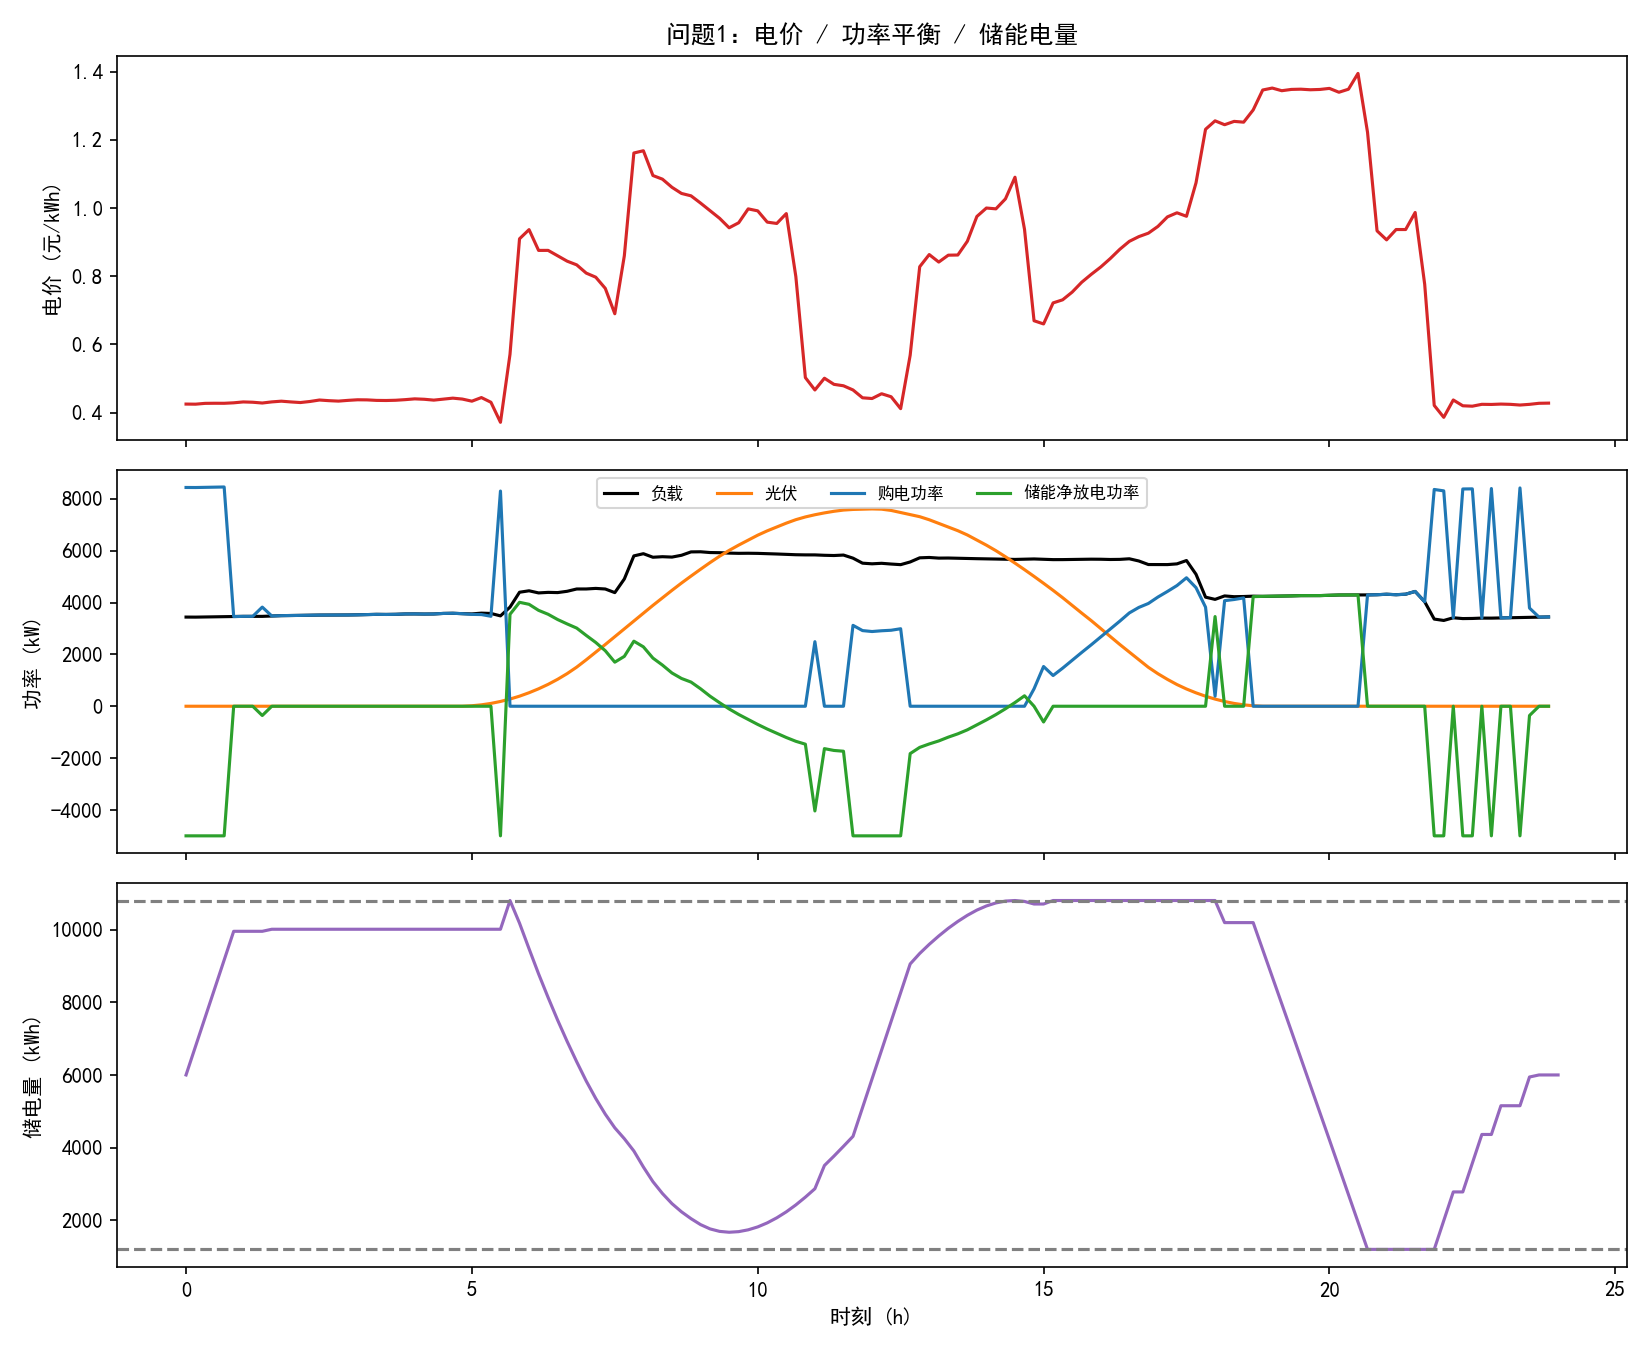
\includegraphics[width=0.85\textwidth]{problem1_plot.png}
\caption{问题一：电价、功率平衡与储能电量曲线}
\label{fig:q1-curve}
\end{figure}

\subsection{模型检验}\label{sec:q1-check}
对结果做以下校验：(1) 全部 144 个时段 $\min(\text{供电}-\text{负载})=-2.27\times10^{-13}$，
数值上等于 0，电力平衡约束严格满足；(2) 储电量全程 $s_t\in[1200,10800]$，未越界；
(3) 未出现同一时段同时充电与放电的情形（0 例），验证了\cref{asu:no-simultaneous}。

\section{问题二：全年计划购电策略与紧急购电机制}

\subsection{问题分析}
问题二在问题一的基础上，将电价、负荷"每天相同"推广为"电价逐日不变、负荷
与光伏逐日变化"，并新增供电不足时的紧急购电兜底机制。题目任务句为"根据
附件 1 中的电价和附件 2 中的数据，在每天 0:00 制定当天的计划购电策略"，
仅引用附件 1、附件 2，未引用附件 3（光伏预报），且未出现"预测/预报"字样；
相较之下，问题三的任务句明确写为"根据……附件 3 的光伏发电预报数据，在每
天 0:00 制定当天的计划购电策略"。据此本文提出\cref{asu:full-info}。

\subsection{模型假设（问题二特有）}
\begin{assumption}
问题二中，0:00 决策时刻对当天小区负荷与光伏出力具有完全信息，处理方式与
问题一"光伏发电预测功率视为准确"一致；预报与实际之间的偏差留待问题三处理
（依据见~\cref{sec:q1-check}上一段的文本分析）。
\label{asu:full-info}
\end{assumption}

\begin{assumption}
储能电量按日周期在日间衔接：每日 $s_0=s_{144}=6000$~kWh。依据：电价逐日
不变（沿用附件 1 曲线），最优充放电策略应具有以日为周期的稳态特性，跨日
套利的边际收益趋近于 0；同时该假设与"每天 0:00 制定当天计划"的题意一致，
使 334 天可分解为相互独立的日内优化问题。
\label{asu:daily-cyclic}
\end{assumption}

\begin{assumption}（拓展模型 2B）
为检验紧急购电机制的有效性，进一步假设外网正常供电容量存在上限
$\bar G=\rho\times$全年峰值负荷（$\rho\in[0,1]$ 为可调参数），计划购电量
$g_t\le\bar G\cdot\Delta t$；该参数非题目给定，仅用于灵敏度分析。
\label{asu:capacity}
\end{assumption}

\subsection{模型建立}
在\cref{asu:full-info}下，第 $d$ 天（$d=1,\dots,334$，对应 2025.2.1--12.31）
的决策变量为计划购电量 $g_t$、\textbf{紧急购电量 $u_t$}、充放电量 $c_t,d_t$、
储电量 $s_t$。相较问题一，新增变量 $u_t$ 作为电力平衡约束中的追索
(recourse)项，代价为 5 倍电价：
\begin{align}
\min\quad & \sum_{t=0}^{143}\pi_t g_t+5\sum_{t=0}^{143}\pi_t u_t \label{eq:q2-obj}\\
\text{s.t.}\quad
& g_t+u_t+PV_t+d_t-c_t\ge L_t, && t=0,\dots,143 \label{eq:q2-balance}\\
& s_{t+1}=s_t+\eta_c c_t-\frac{d_t}{\eta_d}, && t=0,\dots,143 \label{eq:q2-soc}\\
& 1200\le s_t\le10800 \label{eq:q2-socbound}\\
& 0\le c_t,\,d_t\le833.33 \label{eq:q2-power}\\
& 0\le g_t\le\bar G\cdot\tfrac16,\quad u_t\ge0 \label{eq:q2-gcap}\\
& s_0=s_{144}=6000 \label{eq:q2-cyclic}
\end{align}
式\eqref{eq:q2-balance}--\eqref{eq:q2-cyclic}与问题一形式一致（对应
\cref{asu:daily-cyclic}），仅式\eqref{eq:q2-balance}新增 $u_t$、
式\eqref{eq:q2-gcap}新增计划购电上限（基础模型 2A 取 $\bar G=+\infty$，
拓展模型 2B 取\cref{asu:capacity}中的有限值）。该模型对 $d=1,\dots,334$
独立求解 334 次，价格序列 $\pi_t$ 不随 $d$ 变化，各日仅通过
式\eqref{eq:q2-cyclic}解耦。

\subsection{求解方法}
使用 \texttt{cvxpy} 的 \texttt{Parameter} 机制仅构建一次模型，循环替换
$L_t,PV_t,\bar G$ 后以 HiGHS 热启动求解，334 天共需求解 334 次线性规划
（代码见 \texttt{code/problem2.py}）。

\subsection{结果}
\subsubsection{基础模型 2A：全年结果}
全年（334 天）计划购电费为 \num{11806624.21}~元（约 1180.66 万元），
\textbf{紧急购电费恒为 0}。表~\ref{tab:q2-t1}、表~\ref{tab:q2-t2}以
2025-03-20 为例给出表 1、表 2 格式的结果，其余日期结果见
\texttt{result2.xlsx}。

\begin{table}[!htbp]
\caption{问题二示例（2025-03-20）：指定时间段购电量及全天购电量、购电费}\label{tab:q2-t1}\centering
\begin{tabular}{cccccc}
\toprule[1.5pt]
时间段 & 购电量(kWh) & 时间段 & 购电量(kWh) & 时间段 & 购电量(kWh)\\
\midrule[1pt]
10:00--10:10 & 0.0000 & 12:00--12:10 & 479.3120 & 14:00--14:10 & 0.0000\\
16:00--16:10 & 562.2616 & 18:00--18:10 & 366.1427 & 20:00--20:10 & 0.0000\\
\midrule[1pt]
\multicolumn{4}{l}{全天购电量(kWh)} & \multicolumn{2}{c}{64270.8192}\\
\multicolumn{4}{l}{全天购电费(元)} & \multicolumn{2}{c}{38445.8563}\\
\bottomrule[1.5pt]
\end{tabular}
\end{table}

\begin{table}[!htbp]
\caption{问题二示例（2025-03-20）：储能设备指定时间段充放电量及首尾储电量}\label{tab:q2-t2}\centering
\begin{tabular}{ccc}
\toprule[1.5pt]
时间段 & 充电量(kWh) & 放电量(kWh)\\
\midrule[1pt]
0:00--4:00   & 4226.3109 & 0.0000\\
4:00--8:00   & 930.3047  & 6417.2567\\
8:00--12:00  & 5771.6235 & 2777.3772\\
12:00--16:00 & 4630.6903 & 254.7228\\
16:00--20:00 & 0.0000    & 6177.1432\\
20:00--24:00 & 5059.6443 & 2930.2165\\
\midrule[1pt]
\multicolumn{2}{l}{0:00 储电量(kWh)} & 6000.00\\
\multicolumn{2}{l}{24:00 储电量(kWh)} & 6000.00\\
\bottomrule[1.5pt]
\end{tabular}
\end{table}

\begin{table}[!htbp]
\caption{问题二：微网在指定日期的紧急购电量（2A基础模型）}\label{tab:q2-t3}\centering
\begin{tabular}{cccccccc}
\toprule[1.5pt]
\multicolumn{2}{c}{2025.3.20} & \multicolumn{2}{c}{2025.6.21} &
\multicolumn{2}{c}{2025.9.23} & \multicolumn{2}{c}{2025.12.21}\\
\midrule[1pt]
时间段 & 购电量 & 时间段 & 购电量 & 时间段 & 购电量 & 时间段 & 购电量\\
\multicolumn{8}{c}{无（四个指定日期紧急购电量均为 0）}\\
\bottomrule[1.5pt]
\end{tabular}
\end{table}

图~\ref{fig:q2-mar}、图~\ref{fig:q2-dec}给出 2025-03-20（春季）与
2025-12-21（冬季）两个典型日的功率平衡与储能电量曲线：冬季光伏出力弱、
负荷更高，全天购电量（\num{91617.15}~kWh）明显高于春季
（\num{64270.82}~kWh），储能循环也更频繁。

\begin{figure}[!htbp]
\centering
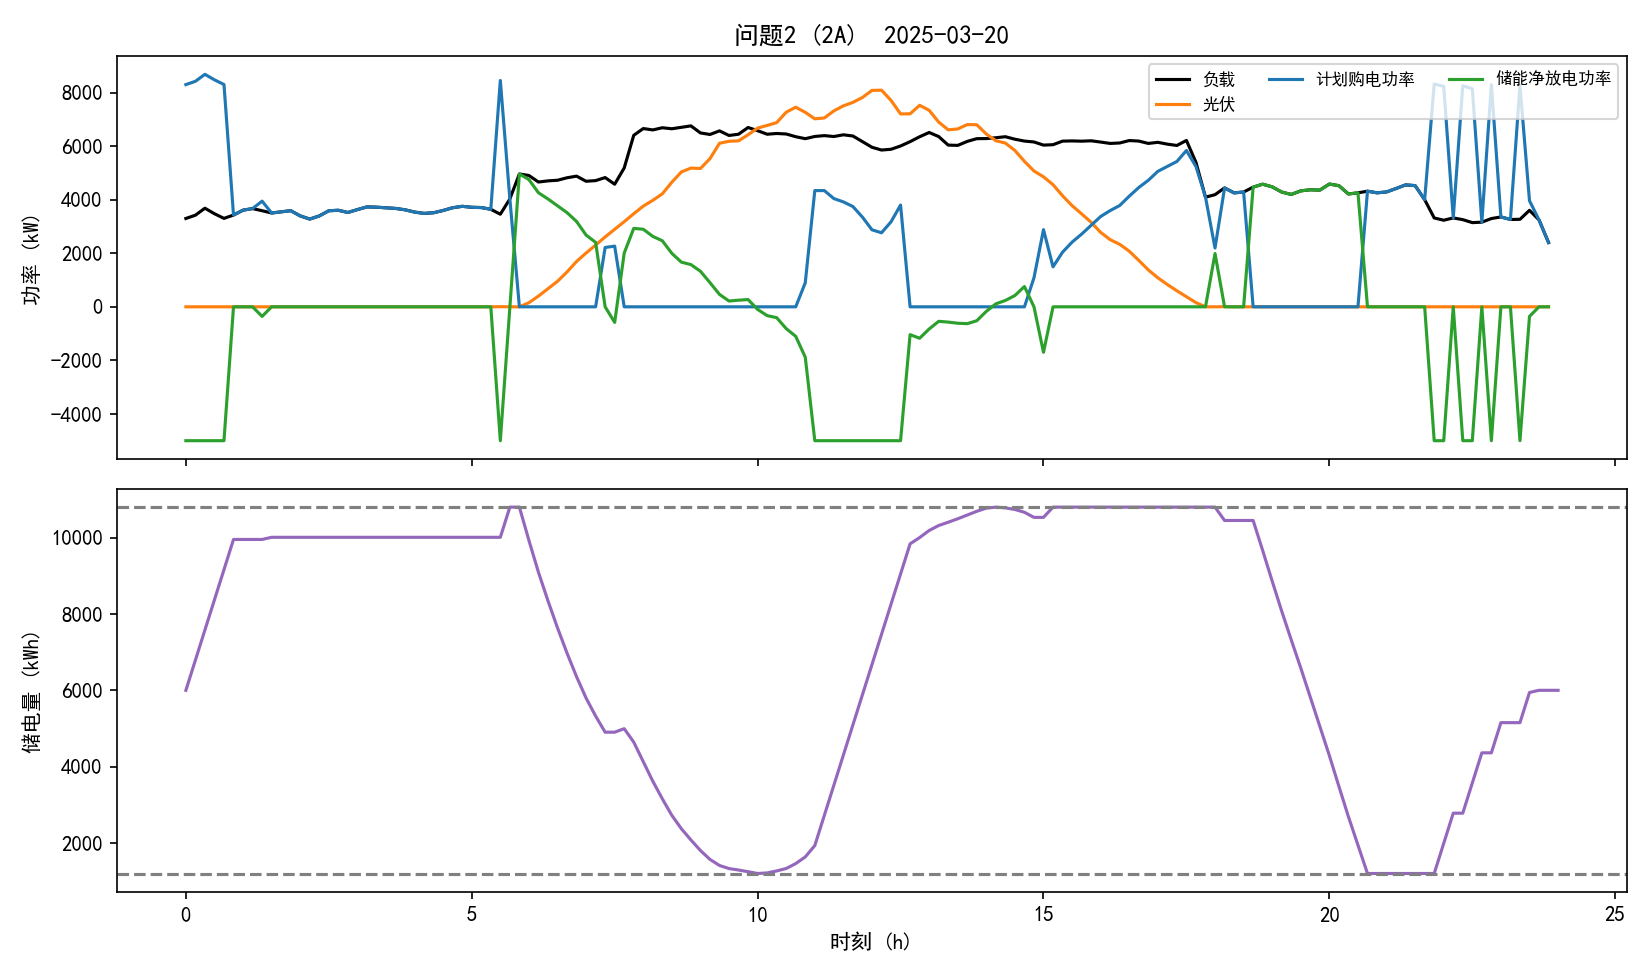
\includegraphics[width=0.85\textwidth]{problem2_plot_20250320.png}
\caption{问题二：2025-03-20 功率平衡与储能电量曲线（2A）}
\label{fig:q2-mar}
\end{figure}

\begin{figure}[!htbp]
\centering
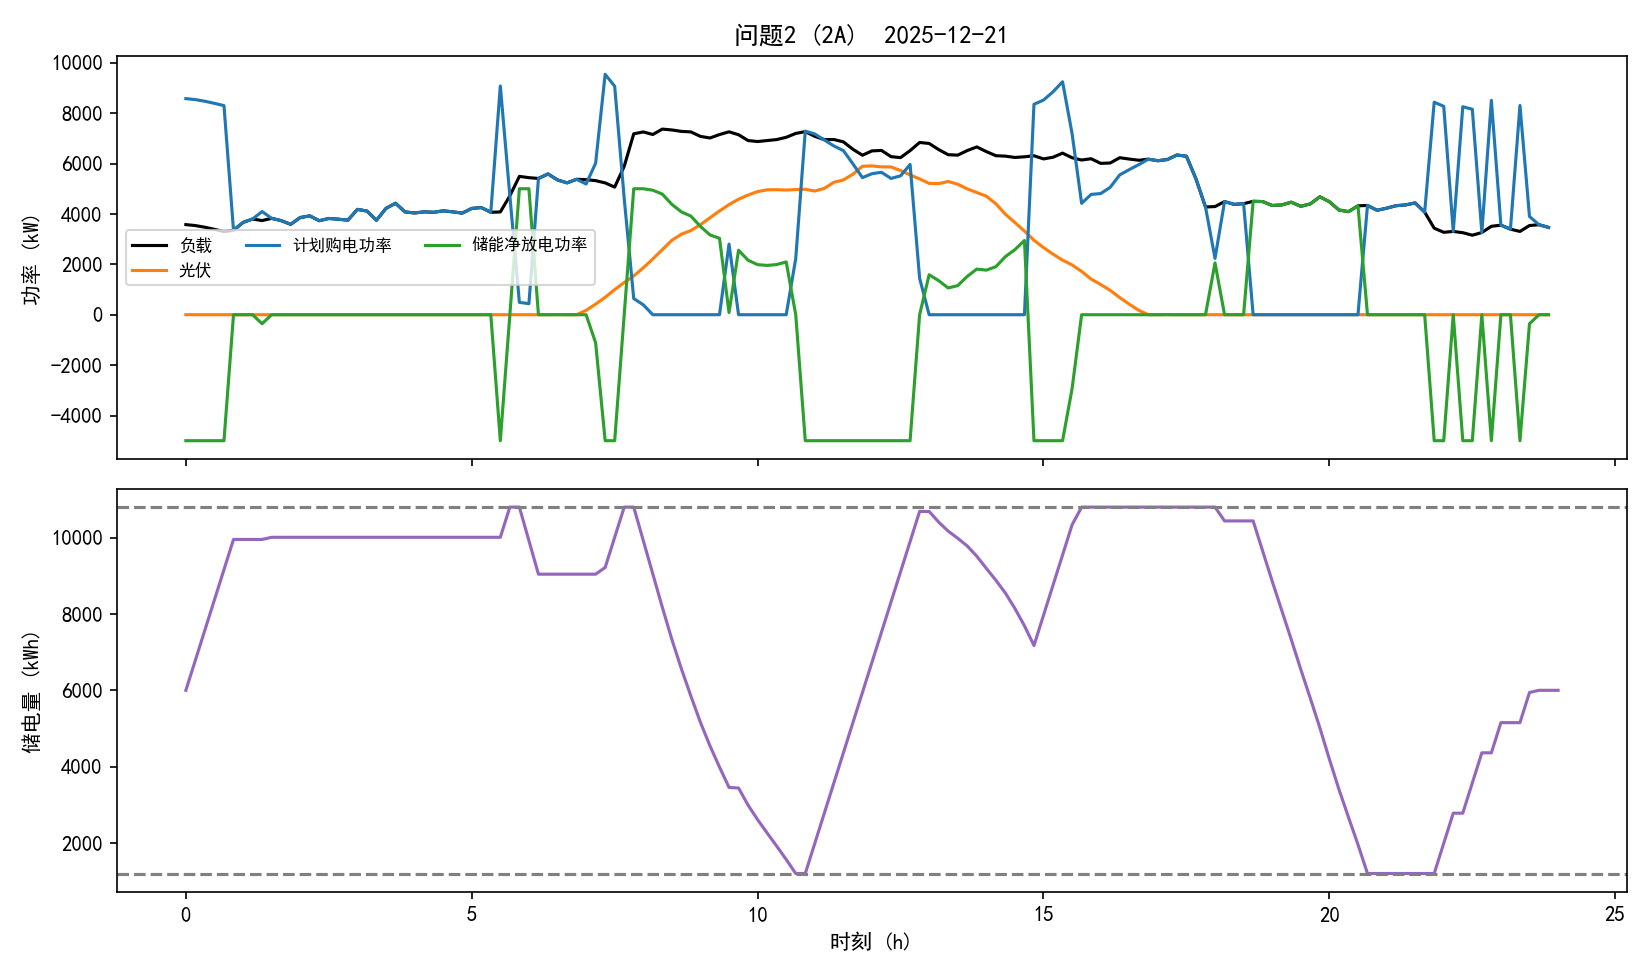
\includegraphics[width=0.85\textwidth]{problem2_plot_20251221.png}
\caption{问题二：2025-12-21 功率平衡与储能电量曲线（2A）}
\label{fig:q2-dec}
\end{figure}

\subsubsection{为什么紧急购电恒为 0}
表~\ref{tab:q2-t3}显示指定日期紧急购电量均为 0，这是\cref{asu:full-info}
（完全信息）与式\eqref{eq:q2-gcap}（2A 模型计划购电量无上限）共同作用的
必然结果：0:00 决策时对当天负荷、光伏完全已知，计划购电量可精确补足
"负荷 $-$ 光伏 $-$ 储能净放电"的缺口，紧急购电条款在数学上不会被触发。

\subsubsection{拓展模型 2B：容量受限下的灵敏度分析}
为验证紧急购电机制并非"死代码"，在\cref{asu:capacity}下对
$\rho=\bar G/(\text{全年峰值负荷})$ 做灵敏度分析（全年峰值负荷为
\num{7978.9}~kW），结果见表~\ref{tab:q2-sens}。

\begin{table}[!htbp]
\caption{问题二拓展模型 2B：外网供电容量灵敏度分析}\label{tab:q2-sens}\centering
\begin{tabular}{ccccc}
\toprule[1.5pt]
$\rho$ & $\bar G$(kW) & 计划购电费(万元) & 紧急购电费(万元) & 紧急天数\\
\midrule[1pt]
0.30 & 2393.7 & 1076.58 & 1283.77 & 273\\
0.40 & 3191.6 & 1270.98 & 399.80  & 246\\
0.50 & 3989.4 & 1307.26 & 53.88   & 66\\
0.60 & 4787.3 & 1248.58 & 0.03    & 2\\
0.70 & 5585.2 & 1201.79 & 0.00    & 0\\
0.80 & 6383.1 & 1185.84 & 0.00    & 0\\
0.90 & 7181.0 & 1181.78 & 0.00    & 0\\
1.00 & 7978.9 & 1181.09 & 0.00    & 0\\
\bottomrule[1.5pt]
\end{tabular}
\end{table}

可见外网容量降至峰值负荷 70\% 以下（$\bar G\lesssim5585$~kW）时，
\num{12000}~kWh/\num{5000}~kW 的储能仍能完全削峰、紧急购电为 0；容量
进一步降至 60\% 时仅有 2 天、8 个时段触发紧急购电（\num{263}~元，可忽略）；
容量降至 50\% 及以下时紧急购电费迅速上升，$\rho=0.30$ 时紧急购电费
（\num{1283.77}万元）已超过计划购电费，凸显 5 倍罚价对总费用的放大效应。
该结果说明：紧急购电机制在\cref{asu:full-info}下于问题二基础模型中确实
不会触发，但其内在逻辑在信息或容量受限情形下是有效、合理的，真正被大量
触发要到问题三（预报存在误差）才会体现。

\subsection{模型检验}\label{sec:q2-check}
对 2A 结果做以下校验（334 天 $\times$ 144 时段，共 \num{48096} 个时段）：
(1) 未出现同一时段同时充电与放电的情形（0 例），验证\cref{asu:no-simultaneous}；
(2) 储电量全程 $s_t\in[1200,10800]$，未越界；(3) $\max(\text{负载}-\text{供电})=5.46\times10^{-12}$，
数值上等于 0；(4) 储能日均充入电量约 \num{18701}~kWh，约为额定容量的 1.56 倍，
说明储能被充分利用（冬季更高，见~\cref{sec:q2-limitation}）。

\subsection{小结与局限性}\label{sec:q2-limitation}
问题二将问题一的单日模型无缝推广至全年 334 天，验证了模型在异质数据下的
可扩展性；紧急购电机制的"零触发"结果经\cref{sec:q1-check}的文本分析与
2B 拓展模型的灵敏度分析双重验证，是完全信息假设下的正确结论而非误差。
局限性：(1) 求解结果显示储能在冬季单日充放电吞吐可达额定容量的 2 倍左右，
模型未考虑循环老化成本，实际部署中需要额外约束或成本项加以限制；
(2) 2B 模型中的容量系数 $\rho$ 为本文自行引入，未在题目中给出。

\section{问题三：多时刻预报下的滚动调整购电策略}
\TODO{建模与求解，待完成。核心思路：0:00 用附件3的0点预报对全天做一次
LP得到"计划"；6/12/18点分别用对应预报，对"剩余时段"重新做一次LP（已过去
时段锁死），并把与原计划的偏差费用（欠购50\%违约、超购1.5倍加价）计入目标
函数，得到"调整"；最终按附件2的真实负荷/光伏结算实际供电缺口与紧急购电
(5倍)。}

\section{问题四：波动电价下的购电策略}
\TODO{复用问题二、三的模型框架，仅将价格输入由附件1替换为附件4的波动电价
重新求解，待完成。}

\section{模型的评价与推广}
\TODO{待问题三、四完成后统一撰写：模型的优点（LP可扩展、求解快速、假设
显式可检验）、局限性（无储能老化成本、日周期假设的适用边界、2B容量参数
的主观性）、可能的推广方向（引入循环老化成本、鲁棒/随机优化处理预测不确定性等）。}

\begin{thebibliography}{9}
\bibitem{lookahead2013}
Look-ahead economic dispatch of microgrids with energy storage, using
linear programming[EB/OL]. ResearchGate, 2013.
\url{https://www.researchgate.net/publication/261040407_Look-ahead_economic_dispatch_of_microgrids_with_energy_storage_using_linear_programming}.

\bibitem{demandresponse2025}
Demand Response Optimization MILP Framework for Microgrids with
DERs[EB/OL]. arXiv:2502.08764, 2025. \url{https://arxiv.org/html/2502.08764v1}.

\bibitem{rollinghorizon2015}
A rolling horizon optimization framework for the simultaneous energy
supply and demand planning in microgrids[J]. Applied Energy, 2015.
\url{https://www.sciencedirect.com/science/article/pii/S0306261915007230}.

\bibitem{cumcmformat}
全国大学生数学建模竞赛论文格式规范.
\end{thebibliography}

\CumcmAIUsed{题意梳理、代码实现（LP建模与\texttt{cvxpy}求解）、结果校验与分析、论文文字与公式排版辅助}

\begin{appendices}
\section{结果文件与代码说明}
本文完整代码见 \texttt{code/} 目录：
\begin{itemize}[leftmargin=2em]
\raggedright
\item[] \texttt{code/problem1.py}：问题一模型实现，输出
\texttt{result1.xlsx}、\texttt{problem1\_summary.txt}。
\item[] \texttt{code/problem2.py}：问题二模型实现（含 2A/2B 两版本与容量
灵敏度分析），输出 \texttt{result2.xlsx}、
\texttt{result2\_capacity\_limited.xlsx}、
\texttt{problem2\_summary.txt}、
\texttt{problem2\_sensitivity\_capacity.txt}（均位于 \texttt{results/} 目录）。
\end{itemize}

\section{问题二核心代码（节选）}
\begin{lstlisting}[language=Python]
g = cp.Variable(144, nonneg=True)   # 计划购电量
u = cp.Variable(144, nonneg=True)   # 紧急购电量
c = cp.Variable(144, nonneg=True)   # 充电量
d = cp.Variable(144, nonneg=True)   # 放电量
s = cp.Variable(145)                # 储能电量
Le = cp.Parameter(144, nonneg=True)   # 当日负载电量
PVe = cp.Parameter(144, nonneg=True)  # 当日光伏电量
Gstep = cp.Parameter(nonneg=True)     # 计划购电每格上限

cons = [
    s[0] == SOC0, s[144] == SOC0,
    s >= SOC_MIN, s <= SOC_MAX,
    s[1:] == s[:-1] + ETA_C * c - d / ETA_D,
    c <= E_STEP_MAX, d <= E_STEP_MAX,
    g <= Gstep,
    g + u + PVe + d - c >= Le,
]
obj = cp.Minimize(price @ g + 5.0 * (price @ u)
                   + EPS_REG * cp.sum(c + d))
\end{lstlisting}
\end{appendices}

\end{document}
